\section{Produto Escalar}

\subsection*{O Produto Escalar}

\begin{frame}[label=vetores2]{O produto escalar}

\begin{defin}
Dados dois vetores $u=(u_1,u_2,\ldots,u_n)$ e $v=(v_1,v_2,\ldots,v_n)$ do $\R^n$, definimos o {\color{blue} produto escalar (ou produto interno)} entre eles por:
\[u\cdot v=u_1v_1+u_2v_2+\cdots+ u_nv_n.\]
\end{defin}

\begin{exe}
Calcule $u\cdot v$, em que $u=(1,2,-3)$ e $v=(-3,5,2)$.
\end{exe}

\end{frame}

\begin{frame}[label=vetores2]

\begin{block}{Propriedades do produto interno} Para quaisquer vetores $u$, ${v}$ e ${w}$ em $\R^n$ e para qualquer número real $\lambda$, valem as propriedades:
			
			\begin{enumerate}
				\item ${u}\cdot {v}={v}\cdot{u}$;
				\item $\lambda( {u}\cdot {v})=(\lambda  {u})\cdot {v}=  {u}\cdot(\lambda {v});$
				\item $( {u}+ {v})\cdot {w}= {u}\cdot {w}+ {v}\cdot {w}$;
				\item $ {u}\cdot {u}=\n{ {u}}^2$.
%				\item $| {u}\cdot {v}|\leq \n{\vect{u}}\n{\vect{v}}$ (desigualdade de Cauchy-Schwartz)
			\end{enumerate}            
		\end{block}
\begin{exe}
Mostre que
\[\|u-v\|^2=\|u\|^2-2u\cdot v+\|v\|^2.\]
\end{exe}

\end{frame}

\subsection*{Ângulo entre vetores}
\begin{frame}[label=vetores2]{Ângulo entre vetores no $\R^2$ e $\R^3$}
	\begin{defin}[ângulo entre vetores] Dados dois vetores $\vt{u}$ e $\vt{v}$, no $\R^2$ ou $\R^3$, definimos o \dest{ângulo entre $\vt{u}$ e $\vt{v}$} como sendo o menor ângulo formado por seus respectivos representantes com mesma origem.			
		\end{defin}

\begin{center}
\begin{minipage}{0.4\textwidth}
	\begin{tikzpicture}
	\tikzset{>=latex}
	\coordinate (O) at (0,0);
	\coordinate (A) at (1,2);
	\coordinate (B) at (2,0);
	\coordinate (C) at (4,1);
	
	\coordinate (X) at (3,0);
	
	\draw[->,ultra thick] (O) -- (A);
	\node[left] at (A) {$\vect{v}$};
	\draw[->,ultra thick] (O) -- (B);
	\node[below] at (B) {$\vect{u}$};
	
	\pic[draw]{angle = B--O--A};
	\node at (0.7,0.5) {$\theta$};
	

	\end{tikzpicture}
\end{minipage}
\begin{minipage}{0.4\textwidth}
	\begin{tikzpicture}
	\tikzset{>=latex}
	\coordinate (O) at (0,0);
	\coordinate (A) at (-1,-2);
	\coordinate (B) at (2,0);
	
	
	\draw[->,ultra thick] (O) -- (A);
	\node[left] at (A) {$\vect{v}$};
	\draw[->,ultra thick] (O) -- (B);
	\node[above left] at (B) {$\vect{u}$};
	
	\pic[draw]{angle = A--O--B};
	\node at (0.6,-0.6) {$\theta$};

	
	\end{tikzpicture}
\end{minipage}

\end{center}
\end{frame}

\begin{frame}
\begin{prop}Dados  $\vt{u}$ e $\vt{v}$, no $\R^2$ ou $\R^3$, então
		\[\vt{u}\cdot\vt{v}=\n{\vt{u}}\n{\vt{v}}\cos ({\color{red}\theta}),\]
		onde ${\color{red}\theta}$ é o ângulo entre eles.
		
	\end{prop}

\begin{center}
	\begin{minipage}{0.3\textwidth}
		\begin{tikzpicture}
		\tikzset{>=latex}
		\coordinate (O) at (0,0);
		\coordinate (A) at (1,2);
		\coordinate (B) at (2,0);
		\coordinate (C) at (4,1);
		
		\coordinate (X) at (3,0);
		
		\draw[->,ultra thick] (O) -- (A);
		\draw[->,ultra thick] (O) -- (B);
		
		\pic[draw]{angle = B--O--A};
		\node at (0.7,0.5) {${\color{red}\theta}$};
		
		\node at (1,-.5) {$\vect{u}\cdot\vect{v}>0$};
		\end{tikzpicture}
	\end{minipage}
	\begin{minipage}{0.3\textwidth}
		\begin{tikzpicture}
		\tikzset{>=latex}
		\coordinate (O) at (0,0);
		\coordinate (A) at (-1,2);
		\coordinate (B) at (2,0);
		
		
		\draw[->,ultra thick] (O) -- (A);
		\draw[->,ultra thick] (O) -- (B);
		
		\pic[draw]{angle = B--O--A};
		\node at (0.7,0.5) {${\color{red}\theta}$};
		\node at (1,-.5) {$\vect{u}\cdot\vect{v}<0$};
		
		\end{tikzpicture}
	\end{minipage}
	\begin{minipage}{0.3\textwidth}
		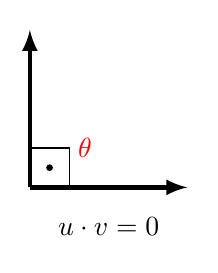
\begin{tikzpicture}
		\tikzset{>=latex}
		\coordinate (O) at (0,0);
		\coordinate (A) at (0,2);
		\coordinate (B) at (2,0);
		
		
		\draw[->,ultra thick] (O) -- (A);
		\draw[->,ultra thick] (O) -- (B);
		
		\draw (0.5,0) -- (0.5,.5) -- (0,0.5);
		\draw[fill] (0.25,.25) circle (1pt);
		\node at (0.7,0.5){${\color{red}\theta}$};
		\node at (1,-.5) {$\vect{u}\cdot\vect{v}=0$};
		\end{tikzpicture}
	\end{minipage}
\end{center}

\end{frame}

\subsection*{Lei dos Cossenos}
\begin{frame}[label=vetores2]


	\begin{exampleblock}{Lei dos Cossenos}
	Seja $ABC$ um triângulo qualquer com lados ${\color{red}a}, {\color{blue}b}$ e ${\color{blue}c}$, então
	\[{\color{red}a^2}={\color{blue}b^2}+{\color{blue}c^2}-2{\color{blue}b c}\cos( {\color{red}\hat{A}}),\]
	onde ${\color{red}\hat{A}}$ é o ângulo oposto ao lado $a$. 
	
	\begin{center}
		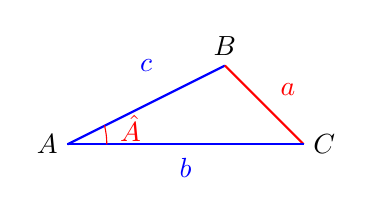
\begin{tikzpicture}
		\draw[thick,blue] (0,0) -- (2,1) ;
		\draw[thick,red] (2,1) -- (3,0) ;
		\draw[thick,blue] (3,0) -- (0,0);
		\node[left] at (0,0) {$A$};
		\node[above] at (2,1) {$B$};
		\node[right] at (3,0) {$C$};
		\node at (2.8,0.7) {${\color{red}a}$};
		\node at (1,1) {${\color{blue}c}$};
		\node at (1.5,-0.3) {${\color{blue}b}$};
		\draw[red] (0.5,0) arc (0:14:1cm);
		\node at (0.8,0.2) {${\color{red}\hat{A}}$};
		\end{tikzpicture}
	\end{center}
\end{exampleblock}
\end{frame}



\begin{frame}[label=vetores2]
\begin{exe}
Determine os ângulo entre os vetores
\begin{enumerate}
\item $\vec{u}=(1,0)$ e $\vec{v}=(\sqrt{3},1)$.

\item $\vec{u}=(2,0,1)$ e $\vec{v}=(1,-2,-1)$.
\end{enumerate}
\end{exe}

\begin{defin}
Dados vetores $u$ e $v$ em $\R^n$, definimos o {\color{blue}ângulo entre $u$ e $v$} como sendo o valor $0\leq \theta\leq \pi$ que satisfaz:
\[\cos(\theta)=\frac{u\cdot v}{\|u\|\, \|v\|}. \] 
\end{defin}

Dizemos que dois vetores são {\color{blue}ortogonais} quando o ângulo entre eles é de $90^\circ$, isto é, quando 
\[u\cdot v=0.\]
\end{frame}


\begin{frame}[label=vetores2]
\begin{casa}
\begin{enumerate}
\item Determine o ângulo entre os vetores $\vec{u}=(2,-3)$ e $\vec{v}=(1,1)$.
\item Um retângulo tem vértices nos pontos $A=(1,2,3)$, $B=(3,6,-2)$ e $C=(0,5,-4)$. Determine o ponto $D$.
\end{enumerate}
\end{casa}
\end{frame}


\subsection*{Produto escalar usando o sympy}
\begin{frame}[label=vetores2,fragile=singleslide]{Produto escalar usando o sympy}

	\begin{footnotesize}
\begin{pyverbatim}
import sympy as sp
import mpmath

u=sp.Matrix([1.12,-3.25,2.07,-1.83 ])
v=sp.Matrix([-2.29,1.72,4.33,-1.54])
uv=u.dot(v)
nu=u.norm()
nv=v.norm()
cos=uv/(nu*nv)
theta=sp.acos(cos)
thetag=round(mp.degrees(theta),2)
\end{pyverbatim}
	\end{footnotesize}	

\begin{pycode}
import sympy as sp
import mpmath as mp

u=sp.Matrix([1.12,-3.25,2.07,-1.83 ])
v=sp.Matrix([-2.29,1.72,4.33,-1.54])
uv=u.dot(v)
nu=u.norm()
nv=v.norm()
cos=uv/(nu*nv)
theta=sp.acos(cos)
thetag=round(mp.degrees(theta),2)
\end{pycode}
Denotando-se os vetores como matrizes colunas, temos:
\[u\cdot v=\pyl{u}\cdot \pyl{v}=\pyl{uv}\]
\[\cos(\theta)\approx\pyl{cos}\Rightarrow \theta\approx\pyl{theta} \text{ rad}\approx \pyl{thetag}^\circ.\]
\end{frame}




